\documentclass[12pt,a4paper]{article}
\usepackage[top=2cm, bottom=2cm, left=2cm, right=2cm]{geometry}

\usepackage{amsmath}
\usepackage{amsfonts}
\usepackage{amssymb}
\usepackage{graphicx}

\usepackage{fontspec}
\setmainfont{Arial}

\usepackage[style=ieee]{biblatex}
\addbibresource{evco.bib}

\usepackage{listings}
\usepackage{longtable}
\usepackage{tabu}
\usepackage{multirow}


\usepackage{hyperref}
\hypersetup{
	colorlinks=true,       % false: boxed links; true: colored links
	allcolors=blue
}

\begin{document}
	
	\begin{titlepage}
		\begin{center}
		\textbf{MEng/MMath/MSc Degree Examinations 2017/18}
		
		\textsc{DEPARTMENT OF COMPUTER SCIENCE}
		
		\vspace{3cm}
		
		\Large
		\textbf{Evolutionary Computation (EVCO)
		Individual Assessment}
	
		\vspace{1.5cm}
		
		\large
		\textbf{Examination Number: Y1403115}
		\end{center}
	\end{titlepage}
	
	
	% 2) Introduction [15 marks]
	\section{Introduction}
	%Intro
	Snake is a 2D, single player action game. The goal of the game is to navigate a snake through a grid, collecting as many food items as possible. The snake grows with each eaten food item. The game is over whenever the snake hits its own body or the wall (in the version of the games where there are walls). 
	
	In this report, a genetic programming(GP) approach is presented for evolving an intelligent snake agent, which achieves as high a score as possible. GP has been proven successful in producing intelligent game agents (\cite{ehlis_application_2000}, \cite{cole_using_2004}, \cite{shichel_gp-robocode:_2005}, \cite{koza_genetic_1992}) and can naturally map the snakes actions and sensing functions to a routine which is efficient and readable.
	
	The report is structured as follows. In \autoref{related_work} the related work in evolutionary algorithms' (EAs) application to games and heuristic and evolutionary approaches for solving the snake game are presented. \autoref{methods} describes the problem and particular approach used to find a solution. \autoref{results} discusses the results obtained from experiments. And \autoref{conclusions} summarises the findings and suggests further work.
	
	\subsection{Realated work} \label{related_work}
	%Game playing EA
	There have been many examples in the literature of using evolutionary algorithms(EA) to produce intelligent game playing agents. Some of the applications include using EAs to find optimal parameters for game controllers: Pac-Mann \cite{gallagher_learning_2003}, The
	Open Racing Car Simulator (TORCS) video game \cite{munoz_multi-objective_2010} and Counter Strike \cite{cole_using_2004}, using EA based optimisation to find a game state weighting function: Tetris \cite{bohm_evolutionary_2018}, using genetic programming(GP) to design a controller for Robocode \cite{shichel_gp-robocode:_2005} and using neuroevolution approach to produce agents, that play a variety of Atari 2600 games  \cite{hausknecht_neuroevolution_2014}.
	
	%Snake playing AI
	Even though there is interest in applying EAs to games in general, there is not much work in using EAs for the snake game. In \cite{kong_automated_nodate} Kong et. al. compares different search algorithms which do not use EAs. They report finding that some algorithms perform slower compared to others but have greater reliability in terms of the snake not crashing before it has eaten all the food. 
	
	Yeh et. al. \cite{yeh_snake_2016} propose a snake controller which uses a weighted sum of rating functions to determine the best move at each time step. The rating functions were the smoothness(number of subsequent moves in the particular direction), space(how many squares can be reached) and distance to food. An EA was used to determine the weights for each rating function. The controllers were evolved in a game with fixed food positions and outperformed a heuristic based approach in the same game. However they could not outperform the heuristic approach in a game with random food positions.
	
	Ehlis \cite{ehlis_application_2000} uses GP to find a routine consisting of the snakes sensing and movement functions, which achieves the maximum score. This approach is very similar to the solution of the Santa Fe Ant problem described in \cite{koza_genetic_1992} because it uses the game agents sensors and actuators directly as a function set in the GA. The paper focuses on finding a function set which allows the snake to achieve the maximum possible score. All successful solutions involved the snake following a particular pattern and not going straight for the food.
	

	% 3) Methods [35 marks]
	\section{Methods} \label{methods}
	
	\subsection{Problem analysis}
	The game environment is a 13 by 13 grid of squares, with walls in all squares with indexes 0 or 13. The snake starts in square (4,10) and its initial length is 11. On each time step the snake moves one square in the direction it is facing. The snakes action allow it to turn(in place) in one of four direction - up, down, right, left, which are defined relative to the grid and not the direction the snake is facing. New food is randomly placed on the squares not occupied by the snake whenever the snake has eaten the current food item. The game ends whenever the snake head enters a square which has a wall or the snakes body or if the snake makes 196 moves without eating any food.  
	
	The GP approach used for the snake game was motivated by Ehlis \cite{ehlis_application_2000} as well as the solution to the Santa Fe Ant problem described in \cite{koza_genetic_1992} and implemented in \cite{noauthor_artificial_nodate}. However there are some subtle differences between these two problems and our snake game. In particular the turning actions of the snake are defined in terms of the global directions and not the direction the snake is facing. This means that the snake can potentially turn at 360 degrees facing its own body and collide with it. This makes the game harder as there is always a danger in one of the squares adjacent to the snakes head. 
	
	It is worth reasoning about which agent behaviour is desirable and which solutions are optimal. A simple optimal solution to the snake game is a Hamiltonian circuit \cite{noauthor_hamiltonian_2017} going through all squares of the grid irrespective of where the food is. This way wherever the food appears the snake will eventually eat it because it is traversing every single square. Ehlis \cite{ehlis_application_2000} reports that all optimal solutions found follow some Hamiltonian path.
	
	Some important qualities for successful agents include avoiding walls, avoiding own body, avoiding dead ends. Furthermore, if the snake agent is not following a Hamiltonian path it is important for it to aim for the food before the timer runs out.
	
	\begin{figure}[h!]
		\centering
		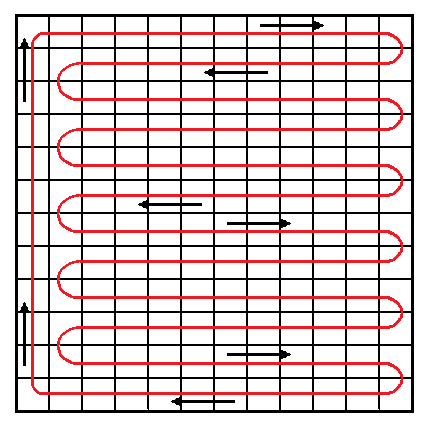
\includegraphics[width=0.7\linewidth]{figures/hamiltonian}
		\caption{Snake game hamiltonian path}
		\label{fig:ham_path}
	\end{figure}
	
		
	\subsection{Choice of representation}
	Each individual in the GP algorithm is represented as a tree of operations from a function set. The function set comprises of terminal and non-terminal nodes. The terminal nodes are turning functions of the snake, which don't have any input or outputs and change the direction of the snake. The non-terminals are the sensing functions of the snake and all take as inputs two other tree elements (terminal or non-terminal) and depending on a condition that they evaluate execute one of their arguments. For example an individual who turns right whenever there is food in the square right of the snake head is shown in \autoref{fig:tree} and would evaluate the expression be equivalent to the python expression \lstinline|if_food_right(changeDirectionRight, changeDirectionUp)|, which executes \lstinline|changeDirectionRight| if there is food in the right square and \lstinline|changeDirectionUp| otherwise. The terminal function set is shown in \autoref{table:terminals}. 
	
	\begin{figure}[h!]
		\centering
		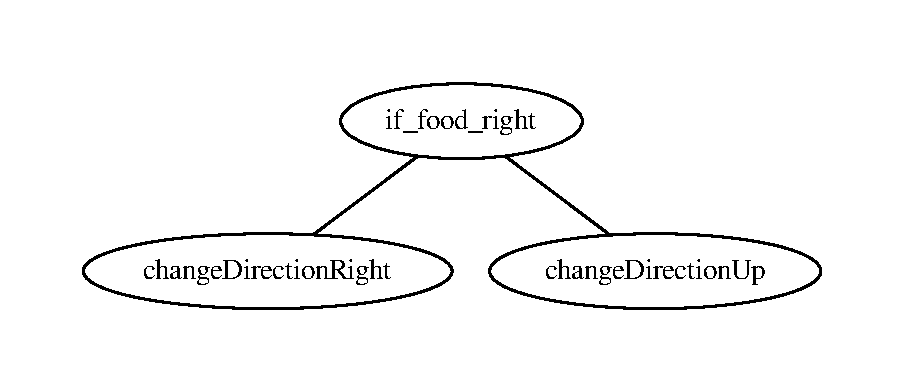
\includegraphics[width=0.7\linewidth]{figures/tree}
		\caption{Example tree representation of an individual.}
		\label{fig:tree}
	\end{figure}
	
	\begin{table}[]
		\centering
		\begin{tabu} to \textwidth {|X[l]|X[l]|}
			\hline
			changeDirectionDown, changeDirectionLeft, changeDirectionRight, changeDirectionUp & Changes the direction the snake is facing. \\  
			\hline
			nothing & The snake remains in the same direction.  \\  
			\hline
		\end{tabu}
		
		\caption{Terminal function set}
		\label{table:terminals}
	\end{table}
	
	Two different non-terminal sets were considered. The first one defines food, wall and tail sensing in all four direction relative to the grid. This means that no mater the direction of travel of the snake, direction up is up on the grid.	This set will be referred to as the absolute non-terminal set and can be see on \autoref{table:absolute-non-terminals}
	
	\begin{table}[h!]
		\centering
		\begin{tabu} to \textwidth {|X[3,l]|X[5,l]|}
			\hline
			if\_food\_up(o1, o2), if\_food\_down(o1, o2), if\_food\_left(o1, o2), if\_food\_right(o1, o2) & If there is food in the line/column of squares to the end of the grid in the specified direction execute first argument otherwise execute second argument\\  
			\hline
			
			if\_wall\_up(o1, o2), if\_wall\_down(o1, o2), if\_wall\_left(o1, o2), if\_wall\_right(o1, o2) & If there is a wall in the square to the specified direction execute first argument otherwise execute second argument\\  
			\hline
			
			if\_tail\_up(o1, o2), if\_tail\_down(o1, o2), if\_tail\_left(o1, o2), if\_tail\_right(o1, o2) & If there is part of the snake's body in the square to the specified direction execute first argument otherwise execute second argument\\  
			\hline
			
			prog2(o1, o2) & Executes its first argument, then executes second argument \\   
			\hline
		\end{tabu}
		
		\caption{Relative non-terminal function set}
		\label{table:relative-non-terminals}
	\end{table}
	
	The other function set defines the above mentioned sensing functions relative to the snake's direction of travel. Because the terminal are defined in terms of the absolute direction, useful routines cannot be constructed. For example if there is danger on the left of the snake, it does not know in which direction relative to the grid it has to turn to avoid it. For this reason additional sensing functions are added, which determine the direction in which the snake is travelling. Furthermore, the snake's body will always be behind it so there is no reason to include sensing for what is behind. This function set will be referred to as the relative non-terminal set (see \autoref{table:relative-non-terminals}).
	
	\begin{table}[h!]
		\centering
		\begin{tabu} to \textwidth {|X[3,l]|X[5,l]|}
			\hline
			if\_food\_ahead(o1, o2), if\_food\_on\_left(o1, o2), if\_food\_on\_right(o1, o2) & If there is food in the line/column of squares to the end of the grid on the specified side of the snake execute first argument otherwise execute second argument\\  
			\hline
			
			if\_wall\_ahead(o1, o2), if\_wall\_on\_left(o1, o2), if\_wall\_on\_right(o1, o2) & If there is a wall in the square on the specified side of the snake execute first argument otherwise execute second argument\\  
			\hline
			
			if\_tail\_ahead(o1, o2), if\_tail\_on\_left(o1, o2), if\_tail\_on\_right(o1, o2) & If there is part of the snake's body in the square on the specified side of the snake execute first argument otherwise execute second argument\\  
			\hline
			
			if\_moving\_up(o1, o2), if\_moving\_down(o1, o2), if\_moving\_left(o1, o2), if\_moving\_right(o1, o2) & If the snake is moving in the specified direction execute first argument otherwise execute second argument\\  
			\hline
			
			prog2(o1, o2) & Executes its first argument, then executes second argument \\   
			\hline
		\end{tabu}
		
		\caption{Absolute non-terminal function set}
		\label{table:absolute-non-terminals}
	\end{table}
	
	This type of representation was chosen because it naturally maps the agents operators to the individual in the GP algorithm. As opposed to using an EA to find some meta parameters for an agent's controller, this approach makes solutions understandable and easier to analyse. It has been successfully applied to the snake game \cite{ehlis_application_2000} and the Santa Fe Ant problem \cite{koza_genetic_1992}, which shares similarities with the snake game. A possible downside to this approach might be that the
	large function set, needed to allow the snake to move and sense its environment, might require a substantial amount of computational resources.
	
	
	\subsection{Fitness evaluation}
	Two different fitness functions were considered and experimented with. The first one (see \autoref{eq:1}) is just the number of food items the snake eats during the run (the score) . 
	
	\begin{equation} \label{eq:1}
		Fitness = score
	\end{equation}
	
	The second fitness function considered is the sum of the score and total number of moves the snake has made. Also the snake's fitness is penalised if it has died because the timer expires. The fitness function can be seen on \autoref{eq:2}, where $steps$ is the total number of moves the snake has made, $timer$ is the value of the timer after the game has finished and $I(timerExpired)$ is a boolean function such that $I(timerExpired) = 1$ if $timerExpired=True$ and $I(timerExpired)=0$ otherwise.
	
	\begin{equation} \label{eq:2}
		Fitness = score + steps - I(timerExpired) * timer
	\end{equation}
	
	The choice of the second evaluation function was motivated by the fact that the Hamiltonian \autoref{fig:ham_path} path solutions do not care about the food. So a possible way to motivate individuals to tend towards such a solution is to award them fitness for traversing the grid. There has to be a trade-off between the pursue of food and the number of moves made, because in earlier generations individual would tend to go in a loop in order to maximise the latter. In order to ensure this does not happen, the penalty is introduced.
	
	\subsection{Evolution operators and parameters}
	On \autoref{table:parameters} the evolution operators and parameters are shown. They were chosen either by reasoning about the problem or empirically - using a few runs. Population size and number of generations were highly restricted by the computational resources available.  

	\begin{table}[h!]
		\centering
		\begin{tabu} to \textwidth {|X[l]|X[l]|}
			\hline
			Population size & 600 \\ \hline  
			Number of generations & 400  \\ \hline 
			Crossover rate & 0.6  \\ \hline  
			Mutation rate & 0.1  \\ \hline    \hline
			
			Initialisation & Ramped half and half \\ \hline
			Initialise min depth & 2  \\ \hline  
			Initialise max depth & 9  \\ \hline  \hline 
			
			Selection & Selection double tournament \\ \hline
			Tournament size & 7  \\ \hline  
			Parsimony size & 1.2  \\ \hline  \hline
			
			Crossover  &  One point crossover with leaf bias \\ \hline
			Leaf crossover probability & 0.1  \\ \hline
			
			Mutation & 	Uniform \\ \hline
			Mutation tree initialisation & Full \\ \hline
			Mutation Min Depth & 1  \\ \hline  
			Mutation Max Depth & 2  \\ \hline  \hline
			
			Bloat control & Static limit on number tree nodes \\ \hline
			Max Nodes & 150  \\ \hline  
		\end{tabu}
		
		\caption{Evolution operators and parameters}
		\label{table:parameters}
	\end{table}
	
	\subsubsection{Initialisation}
	For the initialisation of individuals the ramped half and half method \cite{koza_genetic_1992} is used. It was chosen in order to increase diversity in the initial population. The maximum depth was determined empirically. There cannot be a useful tree with a single element so the minimum was set to 2. Altough, in most cases initialisation produces a good initial population, in some cases bloat occurs, even with bloat control in place (see \autoref{subsubsec:bloat}).
	
	\subsubsection{Selection}
	Initially a simple selection tournament was used for selection. However in order to limit bloat, a selection double tournament was chosen later on. Tournament size was chosen empirically and based on computational resources available. The parsimony was chosen to be relatively small, since there are other bloat control mechanisms used (\autoref{subsubsec:bloat}).
	
	\subsubsection{Crossover}
	The crossover operator was chosen based on the specific problem. Applying crossover to the leaf nodes in the snake's individual representation essentially changes turning action, the agent takes in that branch of the tree. This can rarely lead to beneficial constructs in the offspring, but can lead to good solutions being destroyed. For this reason crossover with a leaf node bias was used, where the probability of choosing a leaf as a crossover point is 0.1 and the probability of choosing a none leaf node is 0.9. The overall crossover rate was chosen empirically to be 0.6.
		
	\subsubsection{Mutation}
	The mutation operator chosen was uniform mutation and uses the full method to construct new trees. In this particular problem mutations can often ruin existing solutions, rather than finding new ones. Furthermore, it is unlikely that randomly generated  trees of great size would yield beneficial constructs. For this reason the maximum depth of trees was set to 2 and the overall mutation probability of the algorithm to 0.1.  
	
	\subsubsection{Bloat control} \label{subsubsec:bloat}
	In order to mitigate the effects of bloat a static limit on the number of nodes in each individual tree was used. This limit was applied to mutation and crossover, so any individual produced by the two operators which had a grater number of nodes was discarded. Limiting tree size was also necessary due to limited computation power. There is also evidence that for the similar Santa Fe Ant problem, there is a greater proportion of solutions in a small tree size \cite{langdon_why_1998}. 
	
	Limiting tree depth was also considered, however sparse deep trees were observed to have a high fitness in some cases. Also it is not clear what the depth limit should be set to without limiting the solution space. 
	
	Although, the size limit is applied to crossover  and mutation, it is not applied to initialisation, meaning that bloat can still occur. However, it is much more unlikely to occur, because of the size limit and the double selection tournament favouring smaller individuals.

    % 4) Results [35 marks]
	\section{Results} \label{results}
	Intro to experiments....
	
	These same operators and parameters were used in all of the experiments unless otherwise indicated in the experiment discussion.
	
	\subsection{Experiment 1}
	The first experiment compared the two evaluation functions from \autoref{eq:1} and \autoref{eq:2}. The absolute non-terminal (\autoref{table:absolute-non-terminals}) and the terminal sets (\autoref{table:terminals}) with the operators and parameters from \autoref{table:parameters} to perform 20 runs with each of the two evaluation functions.
	
	\subsection{Experiment 2}
	
	\subsection{Experiment 3}

    % 5) Conclusions [10 marks]
	\section{Conclusion} \label{conclusions}

	\printbibliography
	
	\appendix
	
\end{document}